\begin{exercises}
\ptwo{Solve the following system of equations by graphing.
\begin{align*}
2x+y &= 4\\
y &= 2x
\end{align*}
\begin{center}
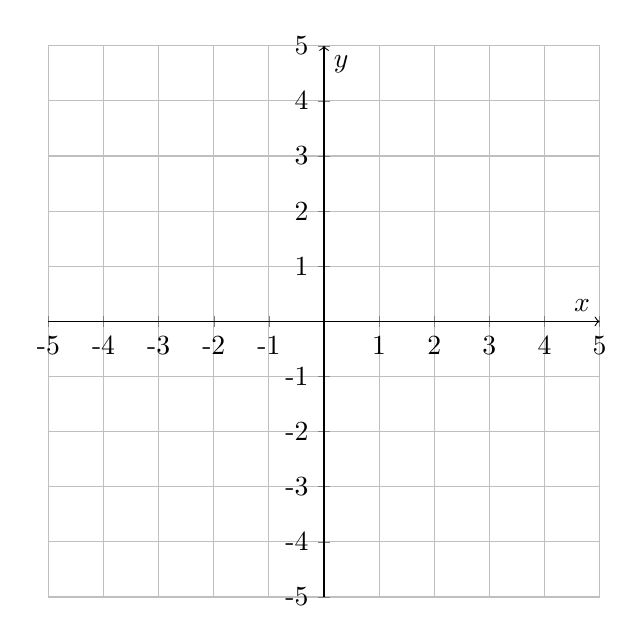
\begin{tikzpicture}
\begin{axis}[
    xmin=-5, xmax=5,
    ymin=-5, ymax=5,
    axis lines=center,
    axis on top=false,
    domain=0:1,
    x=0.7cm,
    y=0.7cm,
    xtick={-10,-9,...,10},
    xticklabels={-10,-9,...,10},
    ytick={-10,-9,...,10},
    yticklabels={-10,-9,...,10},
    axis lines=middle,
    axis line style={->},
    xlabel={$x$},
    ylabel={$y$},
    grid=major
    ]
    
\end{axis}
\end{tikzpicture}
\end{center}}
\ptwo{Solve the following system of equations by graphing.
\begin{align*}
3x-2y &= 2\\
4x+y &= 10
\end{align*}
\begin{center}
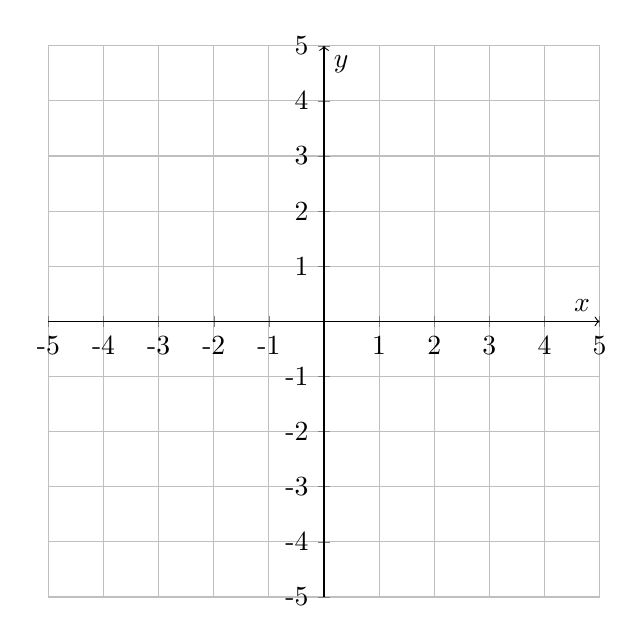
\begin{tikzpicture}
\begin{axis}[
    xmin=-5, xmax=5,
    ymin=-5, ymax=5,
    axis lines=center,
    axis on top=false,
    domain=0:1,
    x=0.7cm,
    y=0.7cm,
    xtick={-10,-9,...,10},
    xticklabels={-10,-9,...,10},
    ytick={-10,-9,...,10},
    yticklabels={-10,-9,...,10},
    axis lines=middle,
    axis line style={->},
    xlabel={$x$},
    ylabel={$y$},
    grid=major
    ]
    
\end{axis}
\end{tikzpicture}
\end{center}}

\ptwo{Solve the following system of equations by graphing.
\begin{align*}
-4 &= 2x-y\\
x &= 2y+1
\end{align*}
\begin{center}
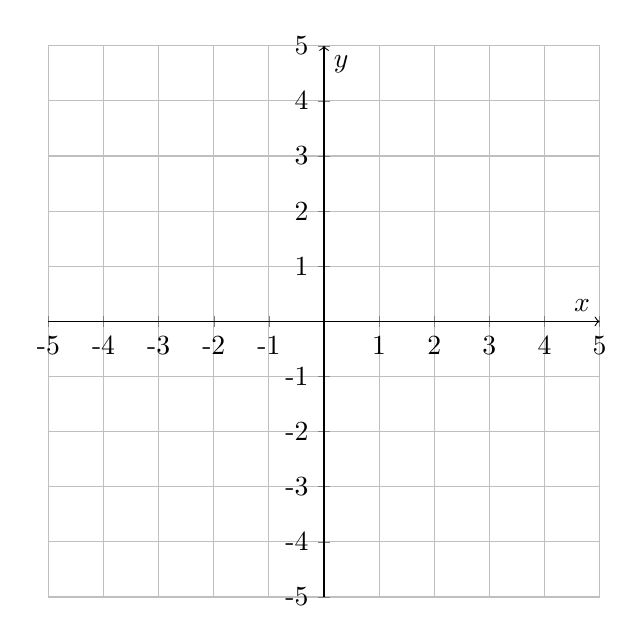
\begin{tikzpicture}
\begin{axis}[
    xmin=-5, xmax=5,
    ymin=-5, ymax=5,
    axis lines=center,
    axis on top=false,
    domain=0:1,
    x=0.7cm,
    y=0.7cm,
    xtick={-10,-9,...,10},
    xticklabels={-10,-9,...,10},
    ytick={-10,-9,...,10},
    yticklabels={-10,-9,...,10},
    axis lines=middle,
    axis line style={->},
    xlabel={$x$},
    ylabel={$y$},
    grid=major
    ]
    
\end{axis}
\end{tikzpicture}
\end{center}}
\ptwo{Solve the following system of equations by graphing.
\begin{align*}
x-3y &= -6\\
x &= -3
\end{align*}
\begin{center}
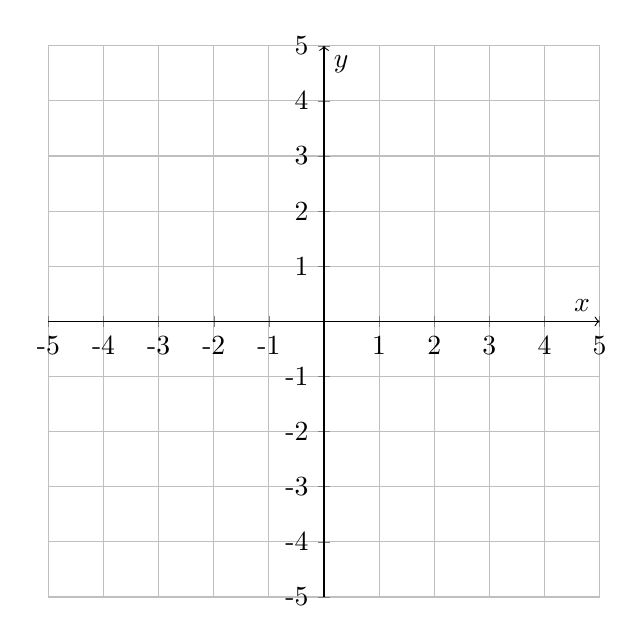
\begin{tikzpicture}
\begin{axis}[
    xmin=-5, xmax=5,
    ymin=-5, ymax=5,
    axis lines=center,
    axis on top=false,
    domain=0:1,
    x=0.7cm,
    y=0.7cm,
    xtick={-10,-9,...,10},
    xticklabels={-10,-9,...,10},
    ytick={-10,-9,...,10},
    yticklabels={-10,-9,...,10},
    axis lines=middle,
    axis line style={->},
    xlabel={$x$},
    ylabel={$y$},
    grid=major
    ]
    
\end{axis}
\end{tikzpicture}
\end{center}}
\vfill
\pagebreak

\textit{In problems 5--13, solve each system of equations by substitution or elimination.}\\
\pthree{
\begin{align*}
3x+5y &= -12\\
x+2y &= -6
\end{align*}
}
\pthree{
\begin{align*}
x-y &= 15\\
y &= -4x
\end{align*}
}
\pthree{
\begin{align*}
x+2y &= 13\\
y+7 &= 4x
\end{align*}
}

\pthree{
\begin{align*}
x-3y &= 0\\
2x-3y &= 6
\end{align*}
}
\pthree{
\begin{align*}
x+y &= 3\\
x-y &= 7
\end{align*}
}
\pthree{
\begin{align*}
3x+y &= -3\\
4x+y &= -4
\end{align*}
}

\pthree{
\begin{align*}
2x+y &= -2\\
5x+3y &= -6
\end{align*}
}
\pthree{
\begin{align*}
5x+2y &= -1\\
4x-5y &= -14
\end{align*}
}
\pthree{
\begin{align*}
y &= -3x+7\\
4x+2y &= 11
\end{align*}
}
\end{exercises}